\documentclass[12pt,b5paper]{ltjsarticle}

%\usepackage[margin=15truemm, top=5truemm, bottom=5truemm]{geometry}
%\usepackage[margin=10truemm,left=15truemm]{geometry}
\usepackage[margin=10truemm]{geometry}

\usepackage{amsmath,amssymb}
%\pagestyle{headings}
\pagestyle{empty}

%\usepackage{listings,url}
%\renewcommand{\theenumi}{(\arabic{enumi})}

\usepackage{graphicx}

%\usepackage{tikz}
%\usetikzlibrary {arrows.meta}
%\usepackage{wrapfig}	% required for `\wrapfigure' (yatex added)
%\usepackage{bm}	% required for `\bm' (yatex added)

% ルビを振る
%\usepackage{luatexja-ruby}	% required for `\ruby'

%% 核Ker 像Im Hom を定義
%\newcommand{\Img}{\mathop{\mathrm{Im}}\nolimits}
%\newcommand{\Ker}{\mathop{\mathrm{Ker}}\nolimits}
%\newcommand{\Hom}{\mathop{\mathrm{Hom}}\nolimits}

%\DeclareMathOperator{\Rot}{rot}
%\DeclareMathOperator{\Div}{div}
%\DeclareMathOperator{\Grad}{grad}
%\DeclareMathOperator{\arcsinh}{arcsinh}
%\DeclareMathOperator{\arccosh}{arccosh}
%\DeclareMathOperator{\arctanh}{arctanh}



%\usepackage{listings,url}
%
%\lstset{
%%プログラム言語(複数の言語に対応,C,C++も可)
%  language = Python,
%%  language = Lisp,
%%  language = C,
%  %背景色と透過度
%  %backgroundcolor={\color[gray]{.90}},
%  %枠外に行った時の自動改行
%  breaklines = true,
%  %自動改行後のインデント量(デフォルトでは20[pt])
%  breakindent = 10pt,
%  %標準の書体
%%  basicstyle = \ttfamily\scriptsize,
%  basicstyle = \ttfamily,
%  %コメントの書体
%%  commentstyle = {\itshape \color[cmyk]{1,0.4,1,0}},
%  %関数名等の色の設定
%  classoffset = 0,
%  %キーワード(int, ifなど)の書体
%%  keywordstyle = {\bfseries \color[cmyk]{0,1,0,0}},
%  %表示する文字の書体
%  %stringstyle = {\ttfamily \color[rgb]{0,0,1}},
%  %枠 "t"は上に線を記載, "T"は上に二重線を記載
%  %他オプション:leftline,topline,bottomline,lines,single,shadowbox
%  frame = TBrl,
%  %frameまでの間隔(行番号とプログラムの間)
%  framesep = 5pt,
%  %行番号の位置
%  numbers = left,
%  %行番号の間隔
%  stepnumber = 1,
%  %行番号の書体
%%  numberstyle = \tiny,
%  %タブの大きさ
%  tabsize = 4,
%  %キャプションの場所("tb"ならば上下両方に記載)
%  captionpos = t
%}



\begin{document}

\hrulefill

次の積分を求めよ。
\begin{equation}
 \int_{1}^{\infty} \frac{1}{x^3+1}\mathrm{d}x
\end{equation}

\dotfill

$f(x)$を次のように定め、
問題の積分を$f(x+1)$の積分として考える。
\begin{equation}
 f(x)=\frac{1}{x^3+1},\qquad
  \int_{1}^{\infty} f(x)\mathrm{d}x
  = \int_{0}^{\infty} f(x+1)\mathrm{d}x
\end{equation}

この積分値を求めるために
複素数上での積分に広げて考える。
具体的には実数の区間$[0,R]$を含む積分路$C$上で
次の式を計算する。
\begin{equation}
 \int_{C} f(z+1)\log{z}\mathrm{d}z
\end{equation}
最終的に$R\to\infty$とするので
$R$は十分に大きい値をとる。($R>2$)

被積分関数$f(z+1)\log{z}=\frac{\log{z}}{(z+1)^3+1}$に対して、
積分経路を次のように考える。

複素平面上において、
$0$中心の半径$R$の円周と、
$0< \delta <\frac{1}{2}$となる十分に小さな$\delta$を利用し
実数直線の正の部分を$+\delta i$だけ平行移動した直線と、
実数直線の正の部分を$-\delta i$だけ平行移動した直線、
$0$中心の十分に小さな$\varepsilon>0$の半径の円周
の4つを作る。
半径$\varepsilon$の円と$+\delta i$だけ平行移動した直線との交点を$P_1\ (Re(P_1)>0)$、
半径$R$の円と$+\delta i$だけ平行移動した直線との交点を$P_2\ (Re(P_2)>0)$、
半径$R$の円と$-\delta i$だけ平行移動した直線との交点を$P_3\ (Re(P_3)>0)$、
半径$\varepsilon$の円と$-\delta i$だけ平行移動した直線との交点を$P_4\ (Re(P_4)>0)$
とする。

$P_1$から$P_2$へ向かう直線を$C_1$、
$P_2$から円周を反時計回りに回って$P_3$へ向かう曲線を$C_2$、
$P_3$から$P_4$へ向かう直線を$C_3$、
$P_4$から円周を時計回りに回って$P_1$へ向かう曲線を$C_4$とする。
この時の複素数$z$の偏角は$0$から$2\pi$の間の値をとるものとする。
($0 \leq \arg{z} \leq 2\pi$)

この4つの積分路をつないで一つの積分路とし、
$C$で表す。
$C=C_1+C_2+C_3+C_4$であり、
各$C_{i}$は次のような曲線である。

\begin{enumerate}
 \item [$C_1$]

       $P_1$から$P_2$へ向かう直線であり、
       この直線上の複素数は
       $z=x+\delta i \ (x\in\mathbb{R})$
       である。

 \item [$C_2$]

       $P_2$から円周を反時計回りに回って$P_3$へ向かう曲線であり、
       円周上の複素数は
       $z=Re^{i\theta} \ (\theta\in\mathbb{R},0\leq\theta\leq2\pi)$
       である。

 \item [$C_3$]

       $P_3$から$P_4$へ向かう直線であり、
       この直線上の複素数は
       $z=x-\delta i \ (x\in\mathbb{R})$
       である。

 \item [$C_4$]


       $P_4$から円周を反時計回りに回って$P_1$へ向かう曲線であり、
       円周上の複素数は
       $z=\varepsilon e^{i\theta} \ (\varepsilon\in\mathbb{R},0\leq\varepsilon\leq2\pi)$
       である。

\end{enumerate}

%%%
%%% 図
%%%
\begin{figure}
\label{fig:hoge}
\centerline{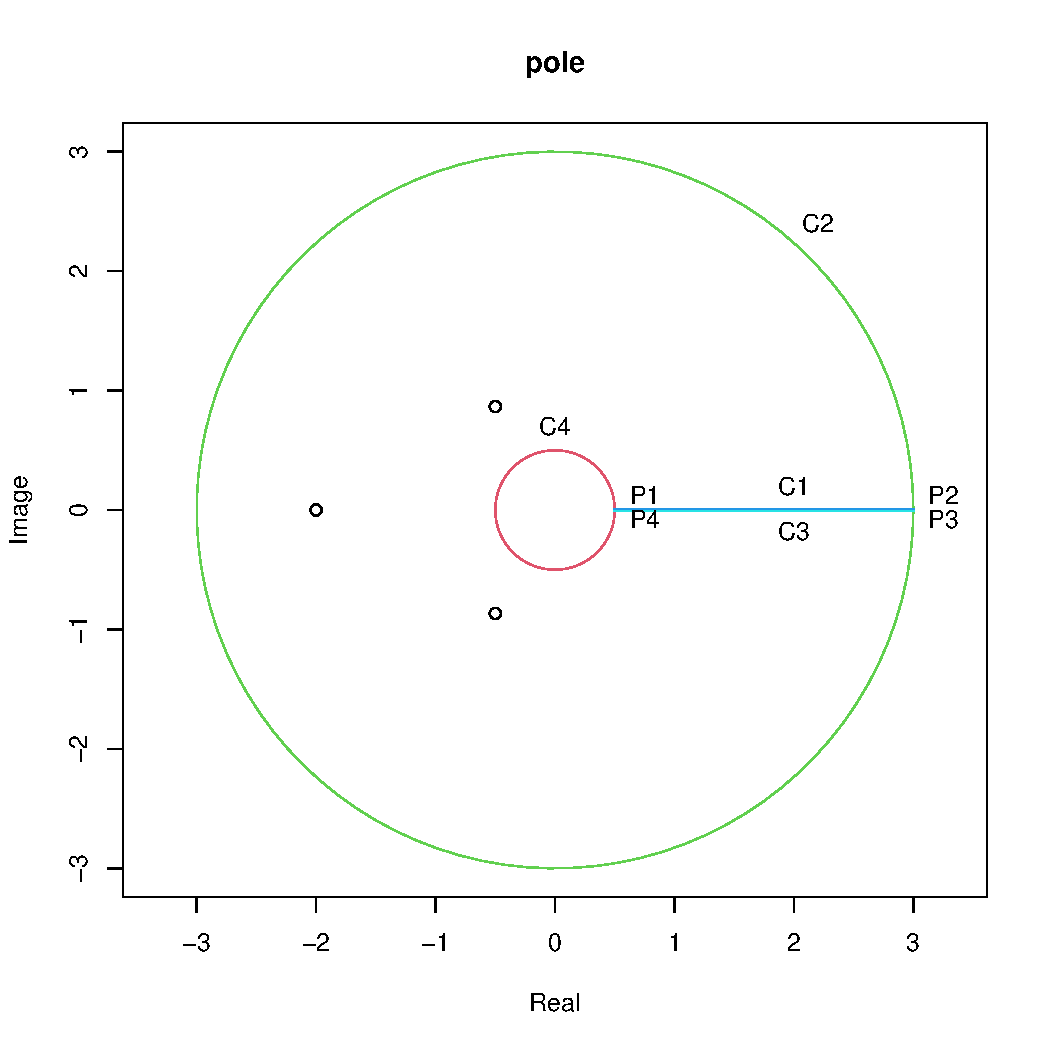
\includegraphics[width=0.5\textwidth]{pole_plot_R.pdf}}
\caption{極の場所と積分経路}
\end{figure}



$C$上の積分は次のような式となる。
\begin{equation}
 \int_{C} f(z)\log{z} \mathrm{d}z
  =
 \int_{C_1} f(z)\log{z} \mathrm{d}z
 +
 \int_{C_2} f(z)\log{z} \mathrm{d}z
 +
 \int_{C_3} f(z)\log{z} \mathrm{d}z
 +
 \int_{C_4} f(z)\log{z} \mathrm{d}z
\end{equation}


$\delta \to 0$と極限をとれば
各積分路上の複素数$z$は次のような式で表される。
\begin{enumerate}
 \item [$C_1$]

       $z=x e^{0i} \ (x:1 \to R)$

 \item [$C_2$]

       $z=Re^{i\theta} \ (\theta : 0\to 2\pi)$

 \item [$C_3$]

       $z=x e^{2\pi i} \ (x:R\to1)$

 \item [$C_4$]

       $z=\varepsilon e^{i\theta} \ (\theta : 2\pi \to 0)$

\end{enumerate}

%%%
%%% 図
%%%

積分路$C$は閉じているので、
留数定理により
積分$\int_{C}f(z+1)\log{z}\mathrm{d}z$は
$C$の内部にある極から求まる。

$f(z+1)\log{z}=\frac{\log{z}}{(z+1)^3+1}$の極は
$(z+1)^3+1=0$を満たし、
$R$が十分に大きく$\varepsilon$が十分に小さいので
全て$C$の内部に存在する。

$w=z+1$として
$w^3+1=0$を満たす複素数を求める。
$w^3=-1=e^{(2n+1)\pi i}$から
$w=e^{\frac{\pi}{3}i},e^{\pi i},e^{\frac{5\pi}{3}i}$
である。
$\omega = e^{\frac{\pi}{3}i}$と置けば、
$w= \omega,\omega^3,\omega^5$であり、
次のような因数分解ができる。
$w^3+1 = (w-\omega)(w-\omega^3)(w-\omega^5)$

%留数定理により
%$\int_{C} f(z+1)\log{z}\mathrm{d}z$
%は
%3つの極$z+1=e^{\frac{\pi}{3}i},e^{\pi i},e^{\frac{5\pi}{3}i}$
%それぞれのの留数から求まる。

オイラーの公式により極は次の複素数と等しい。
\begin{align}
 \omega
 = e^{\frac{\pi}{3}i}
 = \cos{\frac{\pi}{3}}+i\sin{\frac{\pi}{3}}
 =& \frac{1}{2}+\frac{\sqrt{3}}{2}i\\
 \omega^3
 = e^{\pi i}
 = \cos{\pi}+i\sin{\pi}
 =& -1\\
 \omega^5
 = e^{\frac{5\pi}{3}i}
 = \cos{\frac{5\pi}{3}}+i\sin{\frac{5\pi}{3}}
 =& \frac{1}{2}-\frac{\sqrt{3}}{2}i
\end{align}

これらを用いて3つの極の留数を求める。
\begin{align}
 & \mathrm{Res}(f(z+1)\log{z},\omega-1)
  =
 \mathrm{Res}(f(w)\log{(w-1)},\omega)\\
 =&
 \lim_{w\to \omega}(w-\omega)\times \frac{\log{(w-1)}}{w^3+1}
  =
 \lim_{w\to \omega} \frac{\log{(w-1)}}{(w-\omega^3)(w-\omega^5)}\\
 =&
 \frac{\log{(\omega-1)}}{(\omega-\omega^3)(\omega-\omega^5)}
 =
 \frac{\omega\log{(\omega-1)}}{\omega^3(1-\omega^2)(1-\omega^4)}
 =
 -\frac{\omega\log{(\omega-1)}}{(1-\omega^2)(1+\omega)}
 \\
 =& \frac{\log{( e^{\frac{2\pi}{3}i} )}}{3 e^{\frac{2\pi}{3}i}}
 = \frac{\frac{2\pi}{3}i \cdot e^{\frac{\pi}{3}i}}{3 e^{\frac{3\pi}{3}i}}
 = -\frac{\omega}{3}\log{(\omega-1)}
\end{align}

ここで、$\omega= e^{\frac{\pi}{3}i}$に注意して分母を計算する。
\begin{equation}
 (1-\omega^2)(1+\omega)
  =1+\omega -\omega^2-\omega^3
  =2+e^{\frac{\pi}{3}i} -e^{\frac{2\pi}{3}i}
  =3
\end{equation}

また、$(\omega-1)^2$を計算し、$\log{(\omega-1)}$を求める。
\begin{equation}
 (\omega-1)^2
  = ( e^{\frac{\pi}{3}i} + e^{\frac{3\pi}{3}i})^2
  = ( e^{\frac{2\pi}{3}i} )^2
  = e^{\frac{4\pi}{3}i}
\end{equation}
これの対数をとる。
\begin{equation}
 2\log{(\omega-1)}
  = \log{ e^{\frac{4\pi}{3}i} }
  = \frac{4\pi}{3}i
  \quad \Rightarrow \quad
  \log{(\omega-1)} = \frac{2\pi}{3}i
\end{equation}
これにより$\omega-1$の留数は次のように求まる。
\begin{equation}
 \mathrm{Res}(f(z+1)\log{z},\omega-1)
  = -\frac{\omega\log{(\omega-1)}}{(1-\omega^2)(1+\omega)}
  = -\frac{ 2\pi\omega}{9}i
\end{equation}

同様にして$\omega^3-1$の留数も計算する。
\begin{align}
 & \mathrm{Res}(f(z+1)\log{z},\omega^3-1)
 =
 \mathrm{Res}(f(w)\log{(w-1)},\omega^3)\\
 =&
 \lim_{w\to \omega^3}(w-\omega^3)\times \frac{\log{(w-1)}}{w^3+1}
  =
 \lim_{w\to \omega^3} \frac{\log{(w-1)}}{(w-\omega)(w-\omega^5)}\\
 =&
 \frac{\log{(\omega^3-1)}}{(\omega^3-\omega)(\omega^3-\omega^5)}
 =
 \frac{\log{(\omega^3-1)}}{-\omega^3(1+\omega)(1-\omega^2)}
 =
 \frac{\log{(\omega^3-1)}}{3}
\end{align}

$(1+\omega)(1-\omega^2)=3$を用いて分母は$3$であるので、
$(\omega^3-1)^2$を計算し$\log{(\omega^3-1)}$を求める。
\begin{equation}
 (\omega^3-1)^2
  = (e^{\pi i} + e^{\pi i})^2
  = 2e^{2\pi i}
\end{equation}
両辺の対数をとる。
\begin{equation}
 2\log{(\omega^3-1)}
  = \log{2e^{2\pi i}}
  = \log{2} + 2\pi i
  \quad \Rightarrow
  \log{(\omega^3-1)}
  = \frac{1}{2}\log{2} + \pi i
\end{equation}

これにより$\omega^3-1$の留数は次のように求まる。
\begin{equation}
 \mathrm{Res}(f(z+1)\log{z},\omega^3-1)
  =
 \frac{\log{(\omega^3-1)}}{3}
  =
 \frac{1}{6}\log{2} + \frac{\pi}{3} i
\end{equation}


同様にして$\omega^5-1$の留数も計算する。
\begin{align}
 & \mathrm{Res}(f(z+1)\log{z},\omega^5-1)
 =
 \mathrm{Res}(f(w)\log{(w-1)},\omega^5)\\
 =&
 \lim_{w\to \omega^5}(w-\omega^5)\times \frac{\log{(w-1)}}{w^3+1}
  =
 \lim_{w\to \omega^5} \frac{\log{(w-1)}}{(w-\omega)(w-\omega^3)}\\
 =&
 \frac{\log{(\omega^5-1)}}{(\omega^5-\omega)(\omega^5-\omega^3)}
 =
 \frac{\log{(\omega^5-1)}}{-\omega(\omega +1)(1-\omega^2)}
 =
 \frac{\omega^2 \log{(\omega^5-1)}}{3}
\end{align}

$(\omega^5-1)^2$を計算し$\log{(\omega^5-1)}$を求める。
\begin{align}
 (\omega^5-1)^2
  =& (e^{\frac{5\pi}{3}i} + e^{\pi i})^2
  = \left( \frac{1}{2}-\frac{\sqrt{3}}{2}i + (-1) \right)^2
  = \left( -\frac{1}{2}-\frac{\sqrt{3}}{2}i \right)^2\\
  =& (\omega^4)^2
  = \omega^8
  = \omega^2
  = e^{\frac{2\pi}{3}i}
\end{align}
両辺の対数をとる。
\begin{equation}
 2\log{(\omega^5-1)}
  = \log{ e^{\frac{2\pi}{3}i} }
  = \frac{2\pi}{3}i
  \quad \Rightarrow
  \log{(\omega^5-1)}
  = \frac{\pi}{3}i
\end{equation}


これにより$\omega^5-1$の留数は次のように求まる。
\begin{equation}
 \mathrm{Res}(f(z+1)\log{z},\omega^5-1)
  =
 \frac{\omega^2\log{(\omega^5-1)}}{3}
  =
 \frac{\omega^2\pi}{9}i
\end{equation}

%%%%% 3つの留数について
これにより、$C$上の積分は次のようになる。
\begin{align}
 \int_{C} \frac{\log{z}}{(z+1)^3+1}\mathrm{d}z
  =& 2\pi i \left(
            -\frac{2\pi \omega}{9}i
            + \left(\frac{1}{6}\log{2} + \frac{\pi}{3}i\right)
            + \frac{\pi \omega^2}{9}i
           \right)\\
  =&2\pi i \left(
     \frac{1}{6}\log{2}
     + \frac{\pi i}{9} \left( -2\omega + 3 + \omega^2  \right)
  \right)
\end{align}


$C$は4つに分かれるためそれぞれの積分を考える。

$C_1$は直線であり、
$z=x e^{0i}=x \ (x:\varepsilon \to R)$
となる複素数での積分である。
この時$\mathrm{d}z=\mathrm{d}x$である。
\begin{equation}
 \int_{C_1} f(z+1)\log{z}\mathrm{d}z
  =\int_{\varepsilon}^{R} \frac{\log{x}}{(x+1)^3+1}\mathrm{d}x
%  \to \int_{0}^{\infty} \frac{\sqrt{x}}{x^3+1} \mathrm{d}x \ (\varepsilon\to 0, R\to\infty)
\end{equation}

$C_2$は半径$R$の円周上であり、
$z=Re^{i\theta} \ (\theta : 0\to 2\pi)$となる複素数での積分である。
このとき、$\mathrm{d}z = iRe^{i\theta}\mathrm{d}\theta$である。
\begin{align}
 \int_{C_2} f(z+1)\log{z}\mathrm{d}z
 = \int_{0}^{2\pi} \frac{\log{Re^{i\theta}}}{(Re^{i\theta}+1)^3+1} iRe^{i\theta}\mathrm{d}\theta
 = \int_{0}^{2\pi} \frac{ (\log{R}+i\theta)iRe^{i\theta} }{(R e^{i\theta}+1)^3+1} \mathrm{d}\theta
\end{align}


\begin{align}
  \left\lvert
\int_{0}^{2\pi} \frac{ (\log{R}+i\theta)iRe^{i\theta} }{(R e^{i\theta}+1)^3+1} \mathrm{d}\theta
 \right\rvert
  \leq &
 \int_{0}^{2\pi} \frac{ \lvert \log{R}+i\theta \rvert \lvert i \rvert \lvert R \rvert \lvert e^{i\theta} \rvert  }
 { \lvert (R e^{i\theta}+1)^3+1 \rvert} \mathrm{d}\theta
\\
   \leq &
 \int_{0}^{2\pi} \frac{ \lvert \log{R}+i\theta \rvert R }
 { \lvert R e^{i\theta}+1 \rvert^3-1 } \mathrm{d}\theta
 \leq
 \int_{0}^{2\pi} \frac{ (\lvert \log{R} \rvert +2\pi) R }
 { (R -1)^3-1 } \mathrm{d}\theta\\
 = &  \frac{ (\lvert \log{R} \rvert +2\pi) R }{ (R -1)^3-1 }\cdot 2\pi
 \to 0 \quad (R\to \infty)
\end{align}

つまり、$C_2$上の積分は$R\to\infty$において$0$に収束する。
\begin{equation}
 \lim_{R\to\infty}\int_{C_2} f(z+1)\log{z}\mathrm{d}z=0
\end{equation}

次に$C_3$上の積分を考える。
$C_3$は直線であり、
$z=x e^{2\pi i} \ (x:R\to\varepsilon)$
となる複素数での積分である。
この時$\mathrm{d}z=e^{2\pi i}\mathrm{d}x$である。
\begin{align}
  \int_{C_3} f(z+1)\log{z}\mathrm{d}z
   =
  \int_{R}^{\varepsilon} \frac{\log{x e^{2\pi i}}}{(x e^{2\pi i}+1)^3+1}e^{2\pi i}\mathrm{d}x
  =
  \int_{R}^{\varepsilon} \frac{ \log{x} + 2\pi i}{(x+1)^3 +1}\mathrm{d}x\\
  =
 -\int_{\varepsilon}^{R} \frac{ \log{x} }{(x+1)^3 +1}\mathrm{d}x
 - 2\pi i\int_{\varepsilon}^{R} \frac{ 1 }{(x+1)^3 +1}\mathrm{d}x\\
 \to -\int_{0}^{\infty} \frac{ \log{x} }{(x+1)^3 +1}\mathrm{d}x
 - 2\pi i\int_{0}^{\infty} \frac{ 1 }{(x+1)^3 +1}\mathrm{d}x
 \quad (\varepsilon\to 0, R\to\infty)
\end{align}

%よって、$C_3$上の積分は$C_1$上の積分と同じになる。

$C_4$上の積分を考える。
$C_4$は半径$\varepsilon$の円周上であり、
$z=\varepsilon e^{i\theta} \ (\theta : 2\pi \to 0)$となる複素数での積分である。
このとき、$\mathrm{d}z = i \varepsilon e^{i\theta}\mathrm{d}\theta$である。

\begin{equation}
 \int_{C_4}f(z+1)\log{z}\mathrm{d}z
  = \int_{2\pi}^{0}
  \frac{\log{\varepsilon e^{i\theta}}}
  {(\varepsilon e^{i\theta}+1)^3+1} i\varepsilon e^{i\theta}\mathrm{d}\theta
  = \int_{2\pi}^{0} \frac{ (\log{\varepsilon}+i\theta) i\varepsilon e^{i\theta}}
{(\varepsilon e^{i\theta}+1)^3+1} \mathrm{d}\theta
\end{equation}

\begin{align}
 \left\lvert
  \int_{C_4}f(z+1)\log{z}\mathrm{d}z
 \right\rvert
  =&
 \left\lvert
   \int_{2\pi}^{0} \frac{ (\log{\varepsilon}+i\theta) i\varepsilon e^{i\theta}}
{(\varepsilon e^{i\theta}+1)^3+1} \mathrm{d}\theta
 \right\rvert
  \leq 
   \int_{0}^{2\pi} \frac{ \lvert \log{\varepsilon}+i\theta \rvert \lvert i \rvert \lvert \varepsilon \rvert \lvert  e^{i\theta} \rvert}
   { \lvert(\varepsilon e^{i\theta}+1)^3+1\rvert} \mathrm{d}\theta \\
 \leq &
   \int_{0}^{2\pi} \frac{ (\lvert \log{\varepsilon} \rvert + i\theta) \varepsilon }
   { 1- \lvert \varepsilon e^{i\theta}+1 \rvert^3} \mathrm{d}\theta
 \leq
   \int_{0}^{2\pi} \frac{ (\lvert \log{\varepsilon} \rvert + 2\pi) \varepsilon }
   { 1- (1-\varepsilon  )^3} \mathrm{d}\theta\\
 = &
   \frac{ (\lvert \log{\varepsilon} \rvert + 2\pi) \varepsilon }
   { 1- (1-\varepsilon  )^3} \cdot 2\pi
 \to 0 \qquad (\varepsilon\to 0)
\end{align}

よって、$C_4$上の積分は$\varepsilon\to0$において
$0$に収束する。
\begin{equation}
 \lim_{\varepsilon\to 0}\int_{C_4}f(z+1)\log{z}\mathrm{d}z=0
\end{equation}

各$C_{i}$上の積分により$C$上の積分は次のようになる。
\begin{align}
 & \lim_{ \substack{R\to\infty \\ \varepsilon\to 0} }\int_{C} f(z)\log{z}\mathrm{d}z \\
  = &
  % C_1
 \int_{0}^{\infty} \frac{\log{x}}{(x+1)^3+1}\mathrm{d}x
 % C_3
 -\int_{0}^{\infty} \frac{ \log{x} }{(x+1)^3 +1}\mathrm{d}x
 - 2\pi i\int_{0}^{\infty} \frac{ 1 }{(x+1)^3 +1}\mathrm{d}x \\
 =& - 2\pi i\int_{0}^{\infty} \frac{ 1 }{(x+1)^3 +1}\mathrm{d}x
 = - 2\pi i\int_{1}^{\infty} \frac{ 1 }{x^3 +1}\mathrm{d}x
\end{align}
である。


一方、$g(z)=f(z)\log{z}$とすれば、
留数定理より次が成り立つ。
\begin{equation}
  \int_{C} g(z)\mathrm{d}z\\
  = 2\pi i (
  \mathrm{Res}(g,\omega-1)
  +
  \mathrm{Res}(g,\omega^3-1)
  +
  \mathrm{Res}(g,\omega^5-1)
  )
\end{equation}







\hrulefill

\end{document}
